% Copyright 2004 by Till Tantau <tantau@users.sourceforge.net>.
%
% In principle, this file can be redistributed and/or modified under
% the terms of the GNU Public License, version 2.
%
% However, this file is supposed to be a template to be modified
% for your own needs. For this reason, if you use this file as a
% template and not specifically distribute it as part of a another
% package/program, I grant the extra permission to freely copy and
% modify this file as you see fit and even to delete this copyright
% notice. 

\documentclass{beamer}

% There are many different themes available for Beamer. A comprehensive
% list with examples is given here:
% http://deic.uab.es/~iblanes/beamer_gallery/index_by_theme.html
% You can uncomment the themes below if you would like to use a different
% one:
%\usetheme{AnnArbor}
%\usetheme{Antibes}
%\usetheme{Bergen}
%\usetheme{Berkeley}
%\usetheme{Berlin}
%\usetheme{Boadilla}
%\usetheme{boxes}
%\usetheme{CambridgeUS}
%\usetheme{Copenhagen}
%\usetheme{Darmstadt}
%\usetheme{default}
%\usetheme{Frankfurt}
%\usetheme{Goettingen}
%\usetheme{Hannover}
%\usetheme{Ilmenau}
%\usetheme{JuanLesPins}
%\usetheme{Luebeck}
\usetheme{Madrid}
%\usetheme{Malmoe}
%\usetheme{Marburg}
%\usetheme{Montpellier}
%\usetheme{PaloAlto}
%\usetheme{Pittsburgh}
%\usetheme{Rochester}
%\usetheme{Singapore}
%\usetheme{Szeged}
%\usetheme{Warsaw}

\title{Studying Entrepreneurs and Their Environments}

% A subtitle is optional and this may be deleted
%\subtitle{Optional Subtitle}

\author{D. Fehder\inst{1} \inst{2}}
% - Give the names in the same order as the appear in the paper.
% - Use the \inst{?} command only if the authors have different
%   affiliation.

\institute[Rice University] % (optional, but mostly needed)
{
  \inst{1}%
  Rice University
  \and
  \inst{2}%
  TIES Group\\
  MIT Sloan}
% - Use the \inst command only if there are several affiliations.
% - Keep it simple, no one is interested in your street address.

\date{September 14, 2016}
% - Either use conference name or its abbreviation.
% - Not really informative to the audience, more for people (including
%   yourself) who are reading the slides online

\subject{Entrepreneurship}
% This is only inserted into the PDF information catalog. Can be left
% out. 

% If you have a file called "university-logo-filename.xxx", where xxx
% is a graphic format that can be processed by latex or pdflatex,
% resp., then you can add a logo as follows:

% \pgfdeclareimage[height=0.5cm]{university-logo}{university-logo-filename}
% \logo{\pgfuseimage{university-logo}}

% Delete this, if you do not want the table of contents to pop up at
% the beginning of each subsection:

\AtBeginSection[]
{
  \begin{frame}<beamer>{Outline}
    \tableofcontents[currentsection]
  \end{frame}
}

\AtBeginSubsection[]
{
  \begin{frame}<beamer>{Outline}
    \tableofcontents[currentsection]
  \end{frame}
}

% Let's get started
\begin{document}

\begin{frame}
  \titlepage
\end{frame}

\begin{frame}{Outline}
  \tableofcontents
  % You might wish to add the option [pausesections]
\end{frame}

% Section and subsections will appear in the presentation overview
% and table of contents.
\section{Introductions}

\begin{frame}{Welcome!}
  \begin{itemize}
      \item{Take a minute to prepare a very short description including: your name, your year, your major, why you are part of the lab}
      \item{We will go around the room and introduce ourselves}
  \end{itemize}
\end{frame}

\section{What is entrepreneurship? What do we know?}

\begin{frame}{How do we define entrepreneurship?}
\begin{block}{Definition}
The pursuit of opportunity without reference to prior opportunity
\end{block}
  \begin{itemize}
  \item {
    This definition is actually quite general. What do you think it means?
  }
  \item {
    Who would be included in this definition?
  }
  \end{itemize}
\end{frame}

\begin{frame}{There are two types of entrepreneurs}
  \begin{itemize}
      \item{Small to Medium Size Enterprises (SME)}
      \item{Innovation Driven Enterprises (IDE)}
  \end{itemize}
\end{frame}

\begin{frame}{At ESI, we care about IDEs, why?}
  \pause
  \begin{itemize}
      \item{IDEs bring new ideas into the economy
      \begin{itemize}
          \item{Genentech}
          \item{Google}
          \item{Monsanto}
      \end{itemize}
      }
      \item{New ideas are critical for long term economic growth}
  \end{itemize}
\end{frame}

\begin{frame}{The world economy has experienced fantastic growth since 1885}
  \begin{columns}[T]
    \begin{column}{7cm}
% Your image included here
    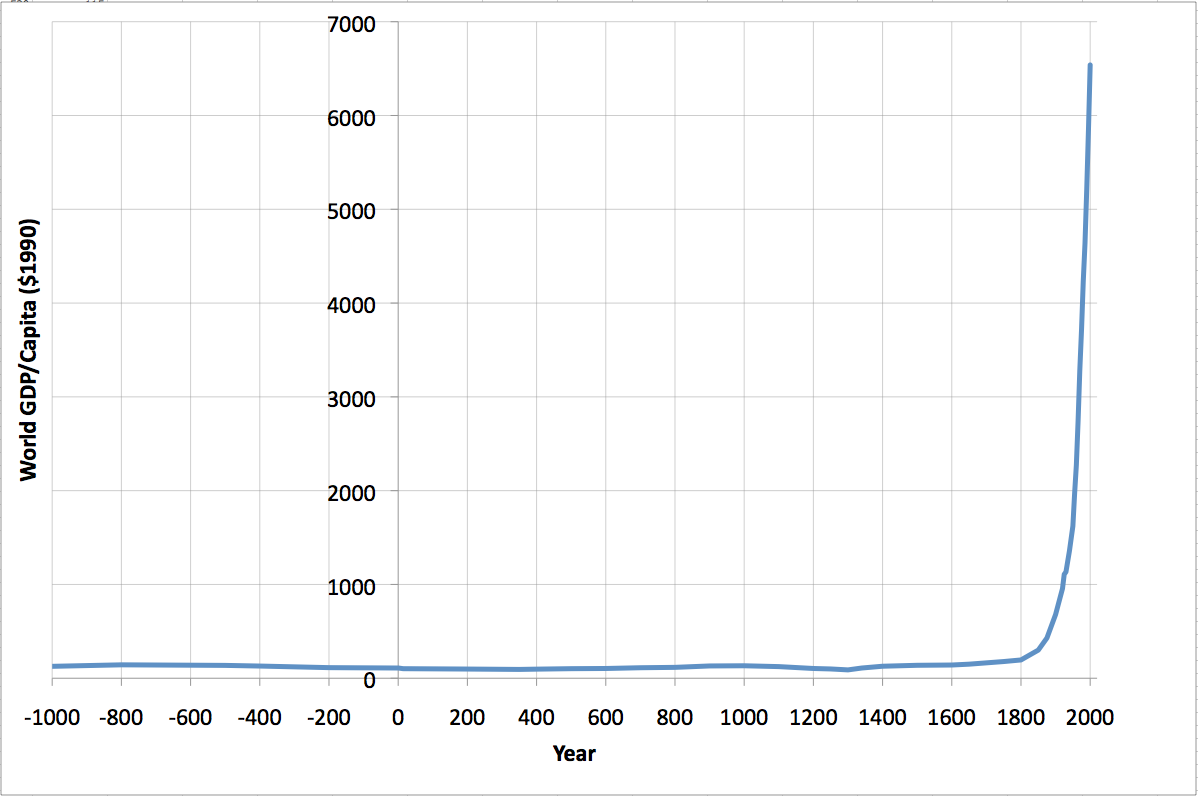
\includegraphics[width=7cm]{WorldGrowth.png}
    \end{column} 
    \begin{column}{.5\textwidth}
    \begin{itemize}
        \item{What do you think changed in the 1880s?
        \pause
        }
        \item{
        The marriage of science and industry 
        }
    \end{itemize}
    \end{column}
  \end{columns}
\end{frame}

\begin{frame}{In 1915, what was the most innovative place in the U.S.?}
  \begin{columns}[T]
    \begin{column}{6cm}
% Your image included here
    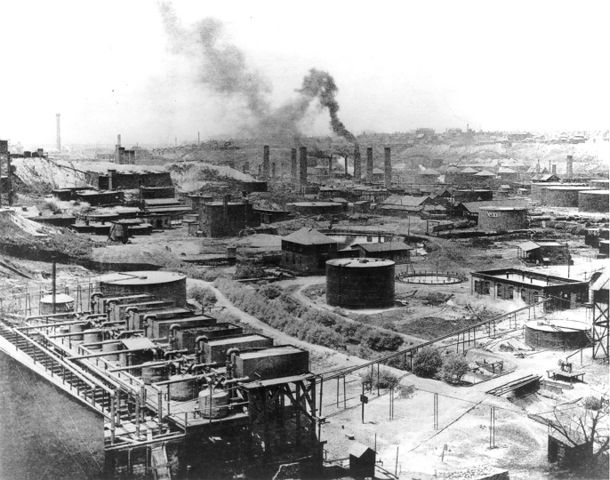
\includegraphics[width=6cm]{Standard_Oil.jpg}
    \end{column} 
    \begin{column}{.5\textwidth}
    \begin{itemize}
        \item{There is a hint in the picture to the left. Guesses?
        \pause
        }
        \item{
        That is the first refinery built by Standard Oil in . . . 
        \pause
        }
        \item{Cleveland. For nearly 50 years, Cleveland was the home to the "second industrial revolution" in the U.S.:
        \begin{itemize}
            \item{Petrochemicals}
            \item{Mechanized Machinery}
        \end{itemize}
        }
    \end{itemize}
    \end{column}
  \end{columns}
\end{frame}


\begin{frame}{How did Silicon Valley become, Silicon Valley?}
\pause
 \begin{itemize}
    \item{Shockley's Mother}
    \item{Smart bets on Silicon-based Transistor}
    \item{Universities (i.e. Stanford)}
    \item{Non-competes}
    \item{Early VCs}
    \item{Other factors}
\end{itemize}
\end{frame}

\begin{frame}{Can we make regions more like SV?}
  \begin{itemize}
      \item{What policies are available?}
      \item{What works?}
      \item{We have a surprisingly low level of clear knowledge}
  \end{itemize}
\end{frame}

\begin{frame}{What are the roles of entrepreneurship programs on economic growth}
\begin{itemize}
    \item{Federal, state and local governments spend billions on them}
    \item{how many are there, what is their distribution?}
    \item{Are regions with more of them more likely to have successful entrepreneurs?}
    \item{Do certain types of programs have more of an impact?}
    \item{Do certain programs act together to have more of an impact?}
\end{itemize}
  
\end{frame}


\section{ESI Lab Expectations}

\begin{frame}{The ESI gives you freedom, but we expect a lot in return}
  \begin{itemize}
      \item{You have to be on slack and email at least once a day}
      \item{You cannot drop out of contact for a whole week}
      \item{We expect 24 hour turn-around on any general queries we make}
  \end{itemize}
\end{frame}

\begin{frame}{General FAQ}
  \begin{itemize}
      \item{What if I have a general question about being an RA? $\Rightarrow$ use the \#general channel on slack}
      \item{What if my plans change during the week? $\Rightarrow$ report your changes to your teammates and to one of the Dans}
      \item{What happens if I don't fill out a weekly reflection? $\Rightarrow$ You are showing lack of commitment to the lab and will jeopardize continued employment}
      \item{What other questions should we add?}
  \end{itemize}
\end{frame}

\section{New Projects and Teams}

\begin{frame}{Project Teams}
  \begin{itemize}
      \item{NAICS 1
      \begin{itemize}
          \item{Rayne}
          \item{Sahil}
          \item{Courtney}
      \end{itemize}
      }
      \item{Name Matching
      \begin{itemize}
          \item{Shiyi}
          \item{Jolen}
          \item{Will Brown}
          \item{Kathy}
      \end{itemize}
      }
      \item{Program Identification
      \begin{itemize}
         \item{Rafael}
         \item{Maxine}
         \item{Jonanne}
      \end{itemize}
      }
      \item{NAICS 2
      \begin{itemize}
          \item{Danning}
          \item{Mengjia}
          \item{Vivian}
      \end{itemize}
      }
  \end{itemize}
\end{frame}


\begin{frame}
  THANK YOU
\end{frame}

\end{document}


